\documentclass[12px]{beamer}
\usepackage{graphicx}
\usepackage{caption}
\DeclareCaptionFont{7pt}{\fontsize{7pt}{5pt}\selectfont}
\captionsetup[figure]{font=7pt}

\graphicspath{ {../paper/images} }
\title{Preserving Accents in Real-Time Audio Translation: A Novel Approach for Linguistic Fidelity}
\author{Irfan Wani}
\institute{Lovely Professional University}
\date{26 April 2024}

\begin{document}
\centering
\frame{\titlepage}
\begin{frame}
\frametitle{Introduction}
\begin{figure}
    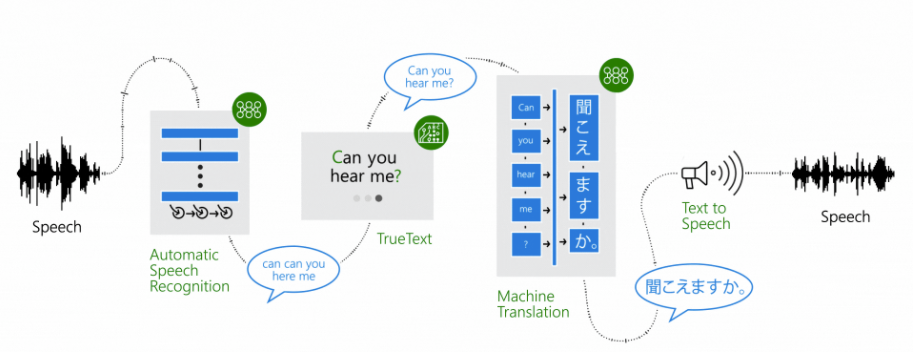
\includegraphics[width=\textwidth]{audiotrans.png}
    \caption{Input is passed to ASR (Automatic Speech Recognition) System to detect the language of input and to convert the speech to text. Any errors are removed and then the result is passed to MT (Machine Translation) model. This converts the input into the desired language.}
\end{figure}
\end{frame}

\begin{frame}
\frametitle{Supported Languages and Models Used}
\begin{figure}
    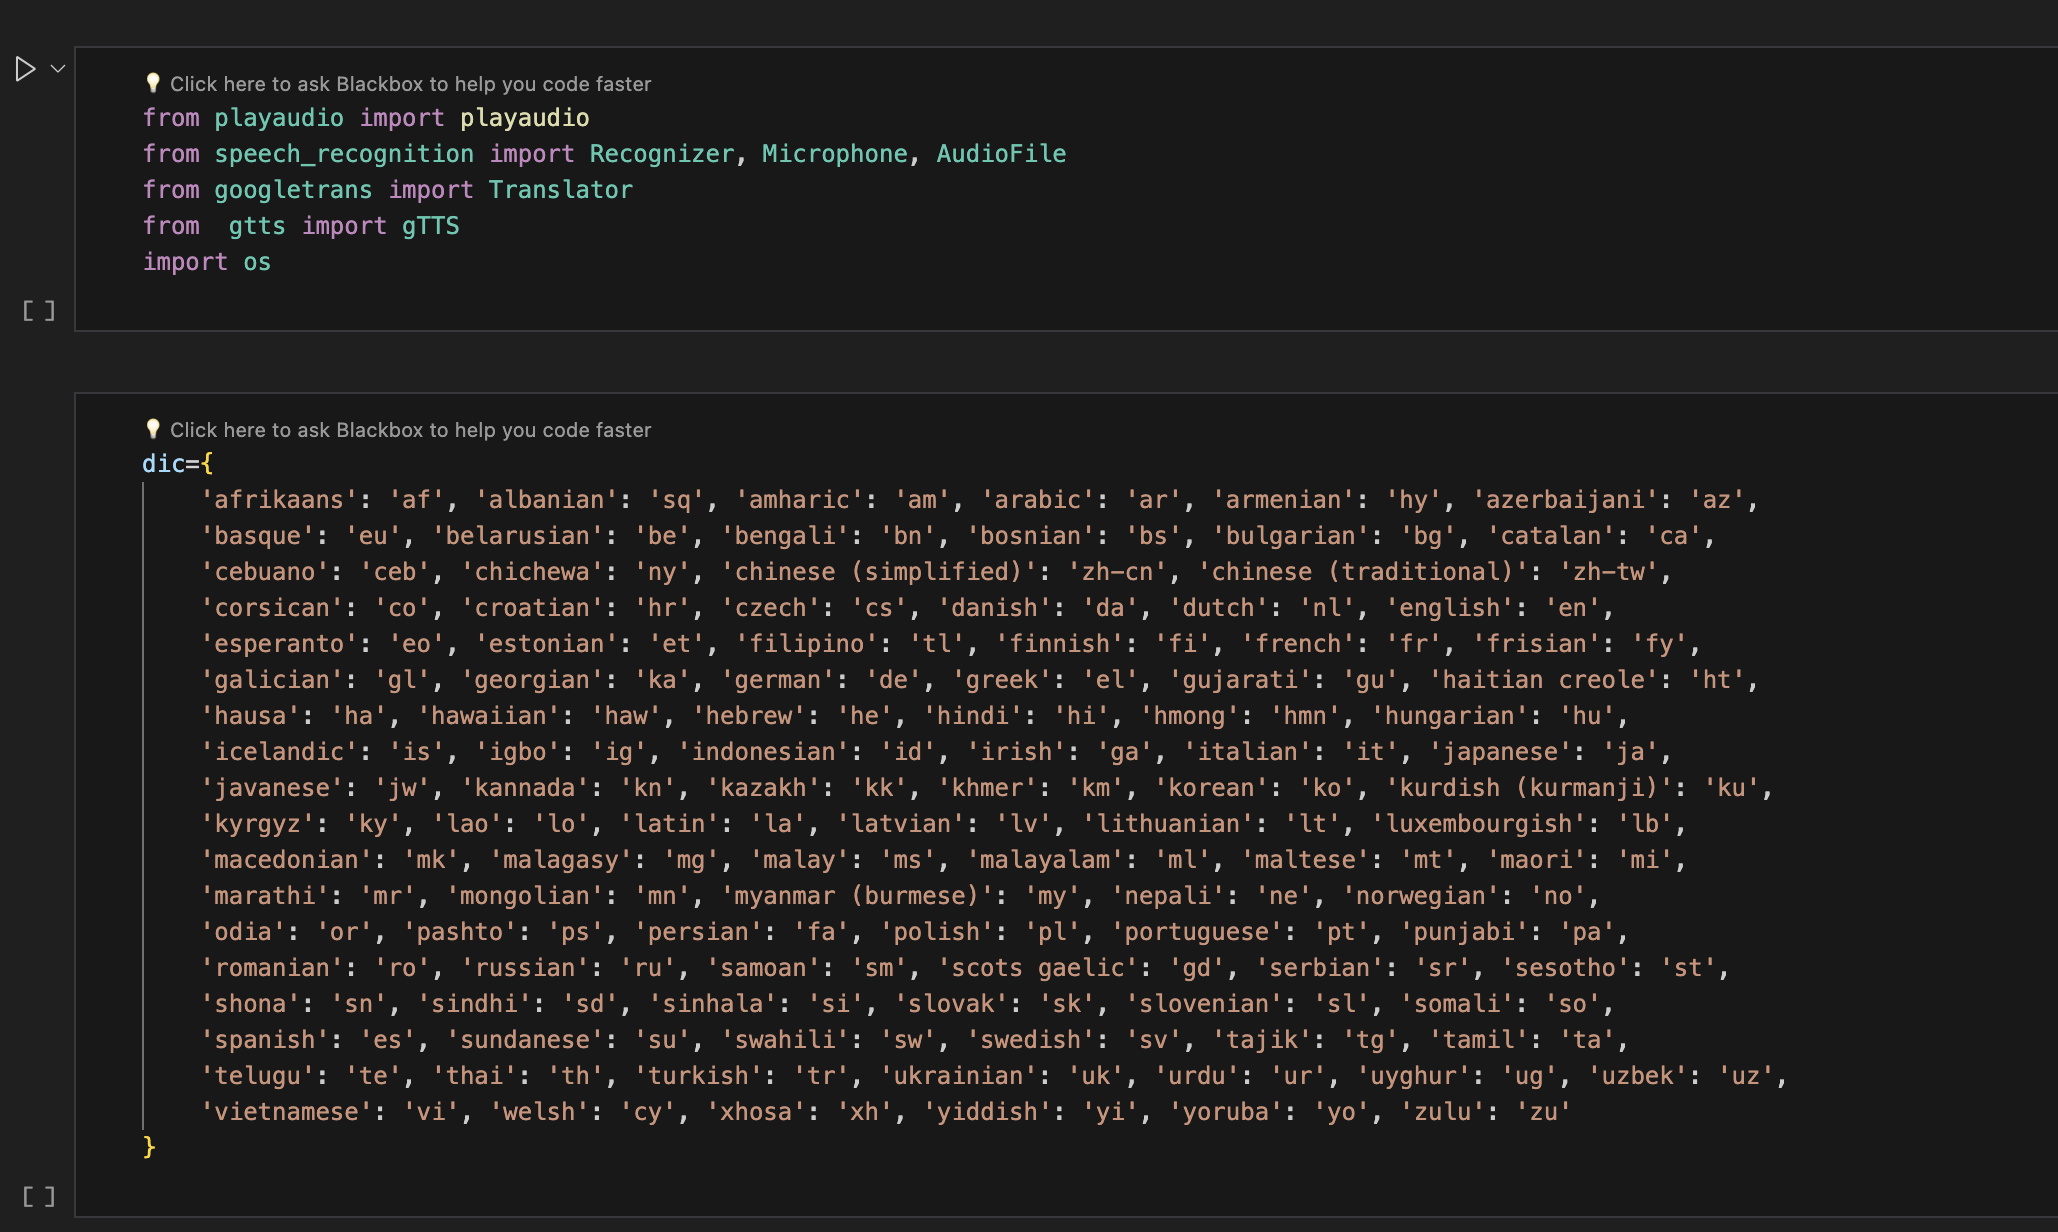
\includegraphics[width=\textwidth]{packagesandlangs.png}
    \caption{Packages like speech recognition, googletrans and google Text to Speech are used in the project. Speech recognition proivdes multiple models, online as well as offline, to convert speech to text. The one used in this project is Whisper from Open AI.}
\end{figure}
\end{frame}

\begin{frame}
\begin{figure}
    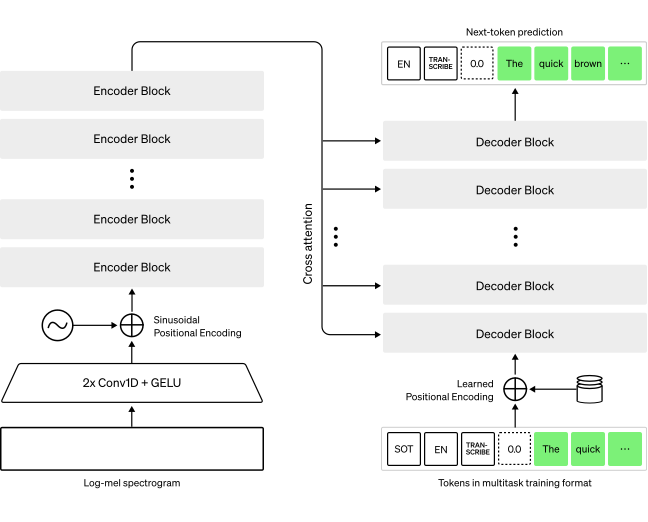
\includegraphics[width=\textwidth]{whisper1.png}
    \caption{Architecture and working of Whisper AI (by Open AI)}
\end{figure}
\end{frame}

\begin{frame}
\begin{figure}
    The Whisper architecture is a simple end-to-end approach. It is implemented as an encoder-decoder Transformer
where the input audio is split into 30-second chunks (parts), then converted into a log-Mel spectrogram, and atlast,
it is passed into an encoder. A decoder is trained to predict the corresponding text caption which performs the
processing along with the steps like, intermixing of special tokens that direct the single model to perform tasks such
as language identification, phrase-level timestamps, multilingual speech transcription, and Translation of speech to
English language.
    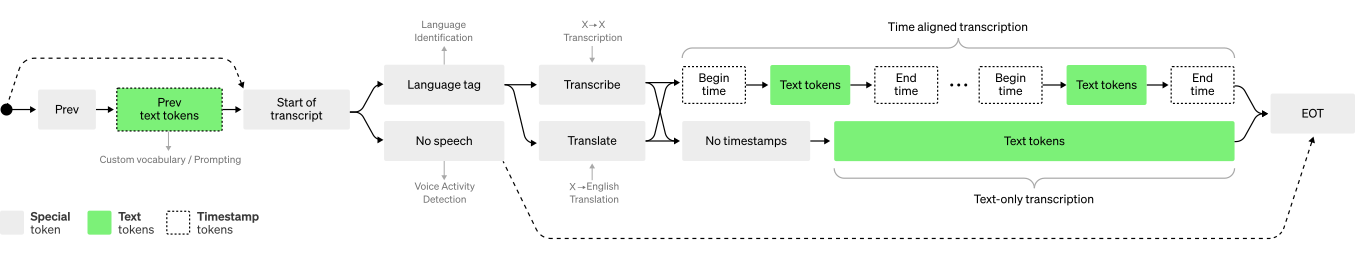
\includegraphics[width=\textwidth]{asr-details.png}
    \caption{ASR (Automatic Speech Recognition) System}
\end{figure}
\end{frame}

\begin{frame}
\begin{figure}
    \frametitle{Machine Translation(MT)}
    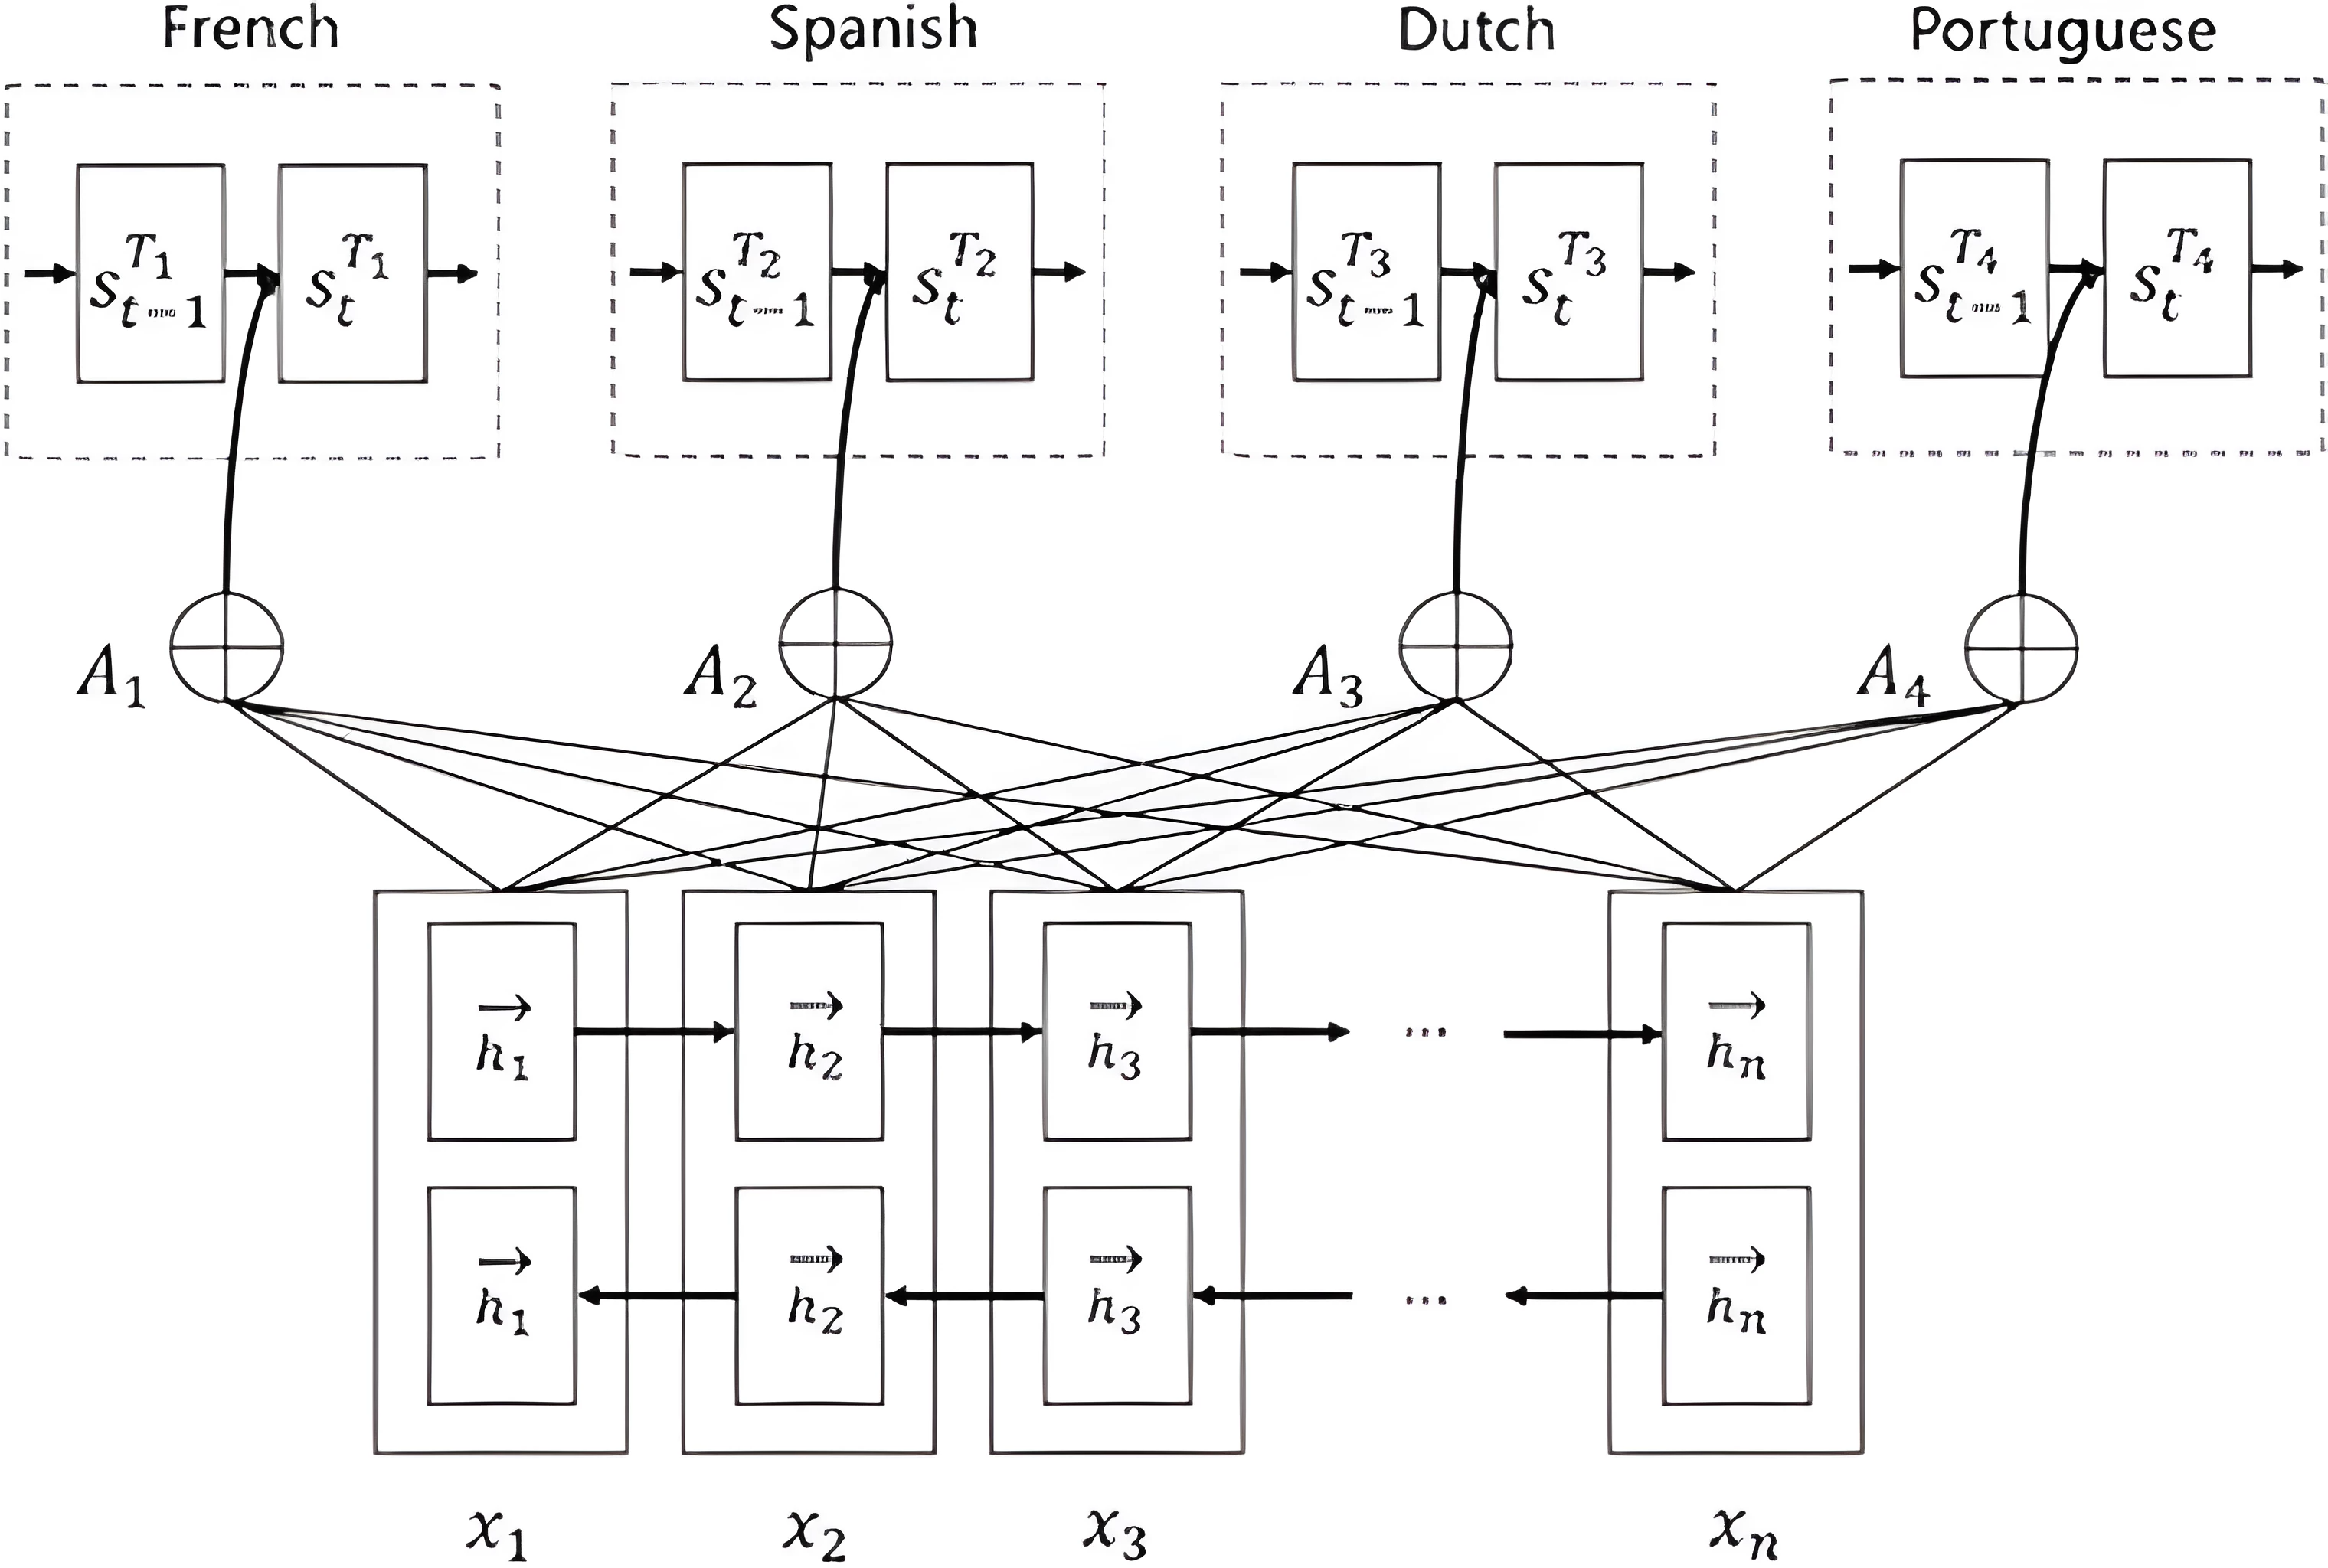
\includegraphics[width=\textwidth]{MT.png}
    \caption{Graphical abstract of Machine Translation}
\end{figure}
\end{frame}

\begin{frame}
\begin{figure}
    \frametitle{Google Translator}
    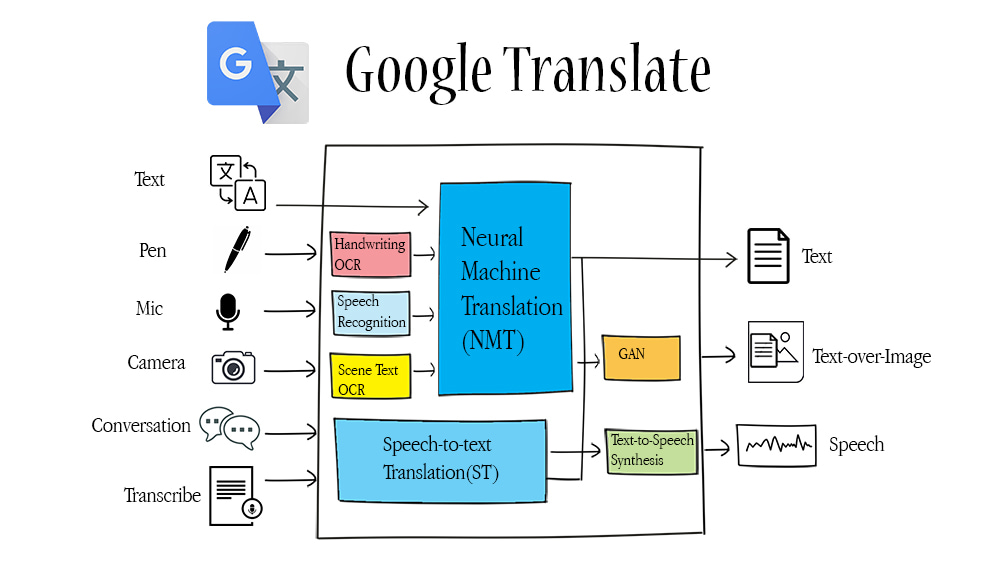
\includegraphics[width=\textwidth]{googletrans.jpeg}
    \caption{Google Translator: Google Translate is an application to translate one language to another in real time. The Google Translate App can translate from handwriting, voice, and camera, and outputs speech and text-over-image. Google Translate uses Google neural machine translation.}
\end{figure}
\end{frame}


\begin{frame}
    \begin{table}[!h]
        \begin{tabular}{|c|c|c|c|c|c|}
            \hline
            \multicolumn{2}{|c|}{\textbf{Accuracy levels of Google Translate for different languages}} \\
            \hline
    
            Spanish & 94\% accurate\\
            \hline
            Korean & 82.5\% accurate\\
            \hline
            Mandarin Chinese & 81.7\% accurate\\
            \hline
            Farsi & 67.5\% accurate\\
            \hline
            Armenian & 55\% accurate\\
            \hline
    
        \end{tabular}
        \caption{Accuracy levels of Google Translate for different target languages from English source content}
    \end{table}
\end{frame}

\begin{frame}
    
\begin{table}[!h]
    \centering
    \begin{tabular}{|c|c|c|c|c|c|}
        \hline
        \textbf{Size} & \textbf{Parameters} & \textbf{English-only model} & \textbf{Multilingual model} & \textbf{Required VRAM} & \textbf{Relative speed}\\
        \hline
        tiny & 39 M & tiny.en & tiny & ~1 GB & ~32x\\
        \hline
        base & 74 M & base.en & base & ~1 GB & ~16x\\
        \hline
        small & 244 M & small.en & small & ~2 GB & ~6x\\
        \hline
        medium & 769 M & medium.en & medium & ~5 GB & ~2x\\
        \hline
        large & 1550 M & N/A & large & ~10 GB & 1x\\
        \hline

    \end{tabular}
    \caption{Available models and languages in Whisper AI}
\end{table}
\end{frame}

\begin{frame}
    \begin{figure}
        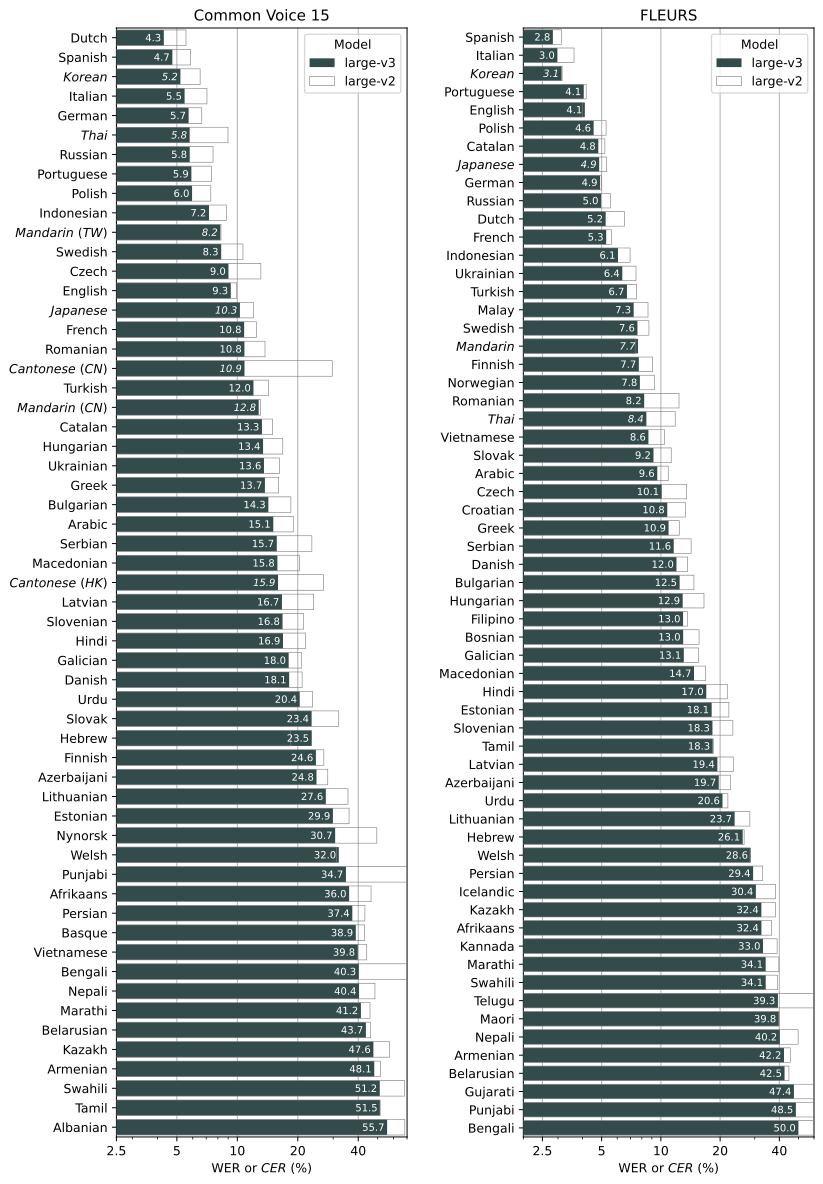
\includegraphics[width=0.5\textwidth]{wer-cer.png}
    \end{figure}
    \end{frame}


\begin{frame}
    \frametitle{References}
    \begin{enumerate}
        \item Jinyu Li - Recent Advances in End-to-End Automatic Speech Recognition [https://arxiv.org/abs/2111.01690]
        \item Whisper AI [https://github.com/openai/whisper]
        \item Alec Radford, Jong Wook Kim, Tao Xu,  Greg Brockman,  Christine McLeavey, Ilya Sutskever - Robust Speech Recognition via Large-Scale Weak Supervision [https://arxiv.org/pdf/2212.04356.pdf]
        \item Jiahuan Li, Shanbo Cheng, Shujian Huang, Jiajun Chen - MT-PATCHER: Selective and Extendable Knowledge Distillation from Large Language Models for Machine Translation [https://arxiv.org/abs/2403.09522/]
        \item Dzmitry Bahdanau, Kyunghyun Cho, Yoshua Bengio - Neural Machine Translation by Jointly Learning to Align and Translate
        [https://arxiv.org/abs/1409.0473/]
        \item https://github.com/Irfanwani/autotranslator.git [code of my project]
        
    \end{enumerate}
\end{frame}
\end{document}